\documentclass{beamer}
\usetheme{Frankfurt}
\usecolortheme{seahorse} %dove
\usepackage{remreset}
\makeatletter
\@removefromreset{subsection}{section}
\makeatother
\setcounter{subsection}{1}

%%aici poate nu am nevoie de tot
\usepackage{listings}
\usepackage{adjustbox}

\usepackage[english]{babel}
\usepackage[T1]{fontenc}
\usepackage{amsmath}
\usepackage{amsfonts}
\usepackage{amssymb}
\usepackage[utf8x]{inputenc}
\usepackage{graphicx}
\usepackage{caption}
\usepackage{subcaption}
\usepackage[font={footnotesize}]{caption}
\usepackage{setspace}
\usepackage{float}
%\usepackage[hidelinks]{hyperref}
\usepackage{wrapfig}
\newcommand*\diff{\mathop{}\!\mathrm{d}}
\setbeamertemplate{caption}[numbered]
\usepackage[authoryear, round]{natbib}
\bibliographystyle{abbrvnat}
\renewcommand{\bibsection}{\subsubsection*{\bibname } }
%aici poate nu am nevoie de tot
\usepackage{soul}
\usepackage{animate}
\usepackage{multicol}

\setbeamertemplate{footline}[frame number]

\title[Robotics] %optional
{\textbf{Through the eyes of RoboFace}}
 
\subtitle{Robotics practical -- final project}
 
\author{Kevin Kiefer, Letiția Elena Pârcălăbescu}
 
\date{the 28\textsuperscript{th} of March 2017}

\begin{document}
\frame{\titlepage}

\begin{frame}
\frametitle{Structure}
\tableofcontents
\end{frame}

\defverbatim[colored]\lstServoConfig{
    \begin{adjustbox}{max size={\textwidth}{\textheight}}
        \begin{lstlisting}[language=C++,basicstyle=\ttfamily,keywordstyle=\color{blue}]
            template<size_t N>
            class ServoConfig
            {
            public:
                ServoConfig(
                    const std::array<int,N> & servoChannel,
                    const std::array<int,N> & servoPos
                );
                // getter & setter
            private:
                std::array<int, N> servoChannel_;
                std::array<int, N> servoPos_;
            };
        \end{lstlisting}
    \end{adjustbox}
}

\defverbatim[colored]\lstServoConstraints{
    \begin{adjustbox}{max size={\textwidth}{\textheight}}
        \begin{lstlisting}[language=C++,basicstyle=\ttfamily,keywordstyle=\color{blue}]
            template<size_t NUM_SERVOS>
            struct ServoConstraints
            {
            public:
                ServoConstraints(
                    int min, int max,
                    const std::array<int, NUM_SERVOS> & channels
                );

                bool isValidChannel(int channel) const;
                bool isValidPosition(int pos) const;

                // isValidChannelArray & isValidPositionArray

                template<size_t N>
                typename std::enable_if<(N <= NUM_SERVOS), bool>::type
                isValidConfig(const ServoConfig<N> & config) const;

            private:
                std::array<int, NUM_SERVOS> channels_;
                int minPos_;
                int maxPos_;
            };
        \end{lstlisting}
    \end{adjustbox}
}

\defverbatim[colored]\lstFaceBackend{
    \begin{adjustbox}{max size={\textwidth}{\textheight}}
        \begin{lstlisting}[language=C++,basicstyle=\ttfamily,keywordstyle=\color{blue}]
            class Face
            {
            public:
                Face(
                    int x_len = 640 , int y_len = 480,
                    float x_weight = 0.5f, float y_weight = 0.5f,
                    const std::string & dev = "/dev/ttyACM0"
                );

                template<size_t N>
                void applyConfig(const ServoConfig<N> & config)

                void happy(bool moveHead = true)
                // more emotions

                void moveHeadX(int x)
                void moveHeadY(int y)
                void moveHead(int x, int y)
            private:
                // ...
            };
        \end{lstlisting}
    \end{adjustbox}
}

\section{Introduction}
\begin{frame}{HumanFace}
	\begin{figure}
		\centering
        \includegraphics[width=\textwidth,height=\textheight,keepaspectratio]{figures/facial_muscles.png}
		\label{fig:facial_muscles}
	\end{figure}
\end{frame}

\begin{frame}{Uncanny Valley}
	\begin{figure}
		\centering
        \includegraphics[width=\textwidth,height=0.8\textheight,keepaspectratio]{figures/uncanny_valley.png}
		\label{fig:uncanny_valley}
	\end{figure}
\end{frame}

\begin{frame}{Uncanny Valley}
	\begin{figure}
		\centering
        \includegraphics[width=\textwidth,height=\textheight,keepaspectratio]{figures/terminator_face.jpg}
		\label{fig:terminator_face}
	\end{figure}
\end{frame}

\section{Hardware}
\begin{frame}{RoboFace}{Hardware}
	\begin{figure}
		\centering
        \includegraphics[width=\textwidth,height=\textheight,keepaspectratio]{figures/RoboFaceNeutral.jpg}
		\label{fig:RoboFaceNeutral}
	\end{figure}
\end{frame}

\begin{frame}{RoboFace}{Hardware}
	\begin{figure}
		\centering
        \includegraphics[width=\textwidth,height=\textheight,keepaspectratio]{figures/RoboFaceBack.jpg}
		\label{fig:RoboFaceBack}
	\end{figure}
\end{frame}

\section{Software}
\begin{frame}{RoboFace}{Software}
    \begin{enumerate}
        \item dependecies: pololu-usb-sdk, RapaPololuMaestro, boost(python), python(2 or 3)
        \item low-lvl code implemented in c++
        \item python api build on top
        \item main workflow implemented in python
    \end{enumerate}
\end{frame}

\begin{frame}{RoboFace}{Software}
    \lstServoConfig
\end{frame}

\begin{frame}{RoboFace}{Software}
    \lstServoConstraints
\end{frame}

\begin{frame}{RoboFace}{Software}
    \lstFaceBackend
\end{frame}

\section{Problem}
\begin{frame}{RoboFace}{Deep Vision Problem}
	\begin{figure}
		\centering
		\vspace*{-18mm}
		\includegraphics[width=0.8\linewidth,angle=270]{figures/roboFace}
		\label{fig:face}
	\end{figure}
\end{frame}

\begin{frame}{RoboFace}{Deep Vision Problem}
		\vspace*{-11.6mm}
		\hspace*{2.85cm}
		\includegraphics[width=0.61\linewidth]{figures/webcam}
\end{frame}

\begin{frame}{Deep Vision}{Short Intro into Neural Networks}
	\centering
	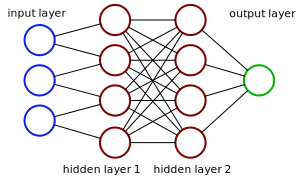
\includegraphics[width=0.61\linewidth]{figures/hiddenLayers}
\end{frame}

\section{Dataset}
\begin{frame}{CelebA Dataset \cite{website}}
\centering
	202.599 images,
	10.177 identities,
	40 attributes per image 
	\begin{figure}
		\centering
		\includegraphics[width=0.9\linewidth]{figures/CelebA}
		\label{fig:celebA}
	\end{figure}
\end{frame}

\begin{frame}{CelebA Dataset}
	\begin{figure}
		\centering
		\includegraphics[width=0.9\linewidth]{figures/CelebAExamples}
		\label{fig:celebAExamples}
	\end{figure}
\end{frame}

\begin{frame}{CelebA Dataset}{Attribute Selection}
	chose 13 labels out of 40 available
	\begin{multicols}{2}
	\begin{enumerate}
	\item Black Hair
	\item Blond Hair
	\item Brown Hair
	\item Eyeglasses
	\item Gray Hair
	\item Male
	\item Mouth Slightly Open
	\item No Beard
	\item Smiling
	\item Straight Hair
	\item Wavy Hair
	\item Wearing Earrings
	\item Wearing Lipstick
	\end{enumerate}
	\end{multicols}
\end{frame}

\section{Own Approach}
\begin{frame}{Own Approach}{Architecture}
	\begin{enumerate}
			\item 	32 of neurons in each convolutional layer
			\item Activations: Relu
			\item 9 x 9 convolution $\rightarrow$ Max Pooling
			\item	7 x 7 convolution $\rightarrow$  Max Pooling
			\item	5 x 5 convolution $\rightarrow$  Max Pooling
			\item	3 x 3 convolution $\rightarrow$  Max Pooling
			\item	3 x 3 convolution $\rightarrow$  Max Pooling
			\item	Dropout(0.25)
			\item	512 Dense
			\item	Dropout(0.5)
			\item	13 Dense
			\item	Sigmoid
			\item	Binary Crossentropy
			\item	Adadelta optimiser
			\item Overall: 125,709 parameters
	\end{enumerate}
\end{frame}

\begin{frame}{Own Approach}{Architecture}
	\hspace*{-1.1cm}
	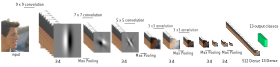
\includegraphics[width=1.2\textwidth]{figures/architecture} 
\end{frame}

\begin{frame}{Own Approach}{How to not do it!}
Without data normalisation: beautiful training curve, BUT...
\hspace*{-2.4cm}
	\includegraphics[height=0.6\textheight]{figures/lossBad} 
\end{frame}

\begin{frame}{Own Approach}{How to not do it!}
... BUT no generalisation capability at all! \\
The predicted classes on the real world images from the robot are: \\
\centering
Male (0.89), No beard (0.76) \\
\centering
\includegraphics[height=0.6\textheight]{figures/failMaleNoBeard} 
\end{frame}

\begin{frame}{Data normalisation}{How to really do it!}
\begin{enumerate}
\item center the eyes
\item resize images to have the same inter ocular distance
\item rotate image to make the inter ocular line look horizontal
\item resize image to 128 x 128 pixels
\item subtract the mean face
\end{enumerate}
\centering
	\includegraphics[height=0.6\textheight]{figures/meanFace} 
\end{frame}

\begin{frame}{Own Approach}{Training Curves}
\hspace*{-2.4cm}
	\includegraphics[height=0.6\textheight]{figures/lossGood} 
\end{frame}

\begin{frame}{Own Approach}{Final Accuracy per Class}
\centering
overall accuracy of 90\%
\centering
	\includegraphics[width=1.1\textwidth]{figures/accuracy_on_classes} 
\end{frame}

\begin{frame}{Exemplary Results}
\centering
'Black Hair', 'Mouth Slightly Open', 'No Beard', 'Smiling', 'Wearing Earrings', 'Wearing Lipstick' \\
\includegraphics[height=0.3\textheight]{figures/leti_normalised110} \\ 
'Black Hair', 'Mouth Slightly Open', 'No Beard', 'Straight Hair', 'Wearing Lipstick' \\
\centering
\includegraphics[height=0.3\textheight]{figures/leti_normalised111} 
\end{frame}

\begin{frame}{Exemplary Results}
'Black Hair', 'Mouth Slightly Open', 'No Beard', 'Smiling', 'Straight Hair', 'Wearing Earrings', \textcolor{red}{'Wearing Lipstick}
 \\
 \centering
\includegraphics[height=0.3\textheight]{figures/leti_normalised24}\\
'Black Hair', \textcolor{red}{'Male'}, 'Straight Hair' -- only 2 out of 45 examples. \\
\centering
\includegraphics[height=0.3\textheight]{figures/leti_normalised0}
\end{frame}

\begin{frame}{Future Potential}
\begin{itemize}
 \item hardware
 \item speech recognition
 \item data acquisition
\end{itemize}

\end{frame}



\section{References}
\begin{frame}
	\frametitle{References}
	\footnotesize
	\bibliography{mybib.bib}
\end{frame}

\end{document}
